%%%%%%%%%%%%%%%%%%%%%%%%%%%%%%%%%%%%%%%%%
% Daily Laboratory Book
% LaTeX Template
%
% This template has been downloaded from:
% http://www.latextemplates.com
%
% Original author:
% Frank Kuster (http://www.ctan.org/tex-archive/macros/latex/contrib/labbook/)
%
% Important note:
% This template requires the labbook.cls file to be in the same directory as the
% .tex file. The labbook.cls file provides the necessary structure to create the
% lab book.
%
% The \lipsum[#] commands throughout this template generate dummy text
% to fill the template out. These commands should all be removed when 
% writing lab book content.
%
% HOW TO USE THIS TEMPLATE 
% Each day in the lab consists of three main things:
%
% 1. LABDAY: The first thing to put is the \labday{} command with a date in 
% curly brackets, this will make a new page and put the date in big letters 
% at the top.
%
% 2. EXPERIMENT: Next you need to specify what experiment(s) you are 
% working on with an \experiment{} command with the experiment shorthand 
% in the curly brackets. The experiment shorthand is defined in the 
% 'DEFINITION OF EXPERIMENTS' section below, this means you can 
% say \experiment{pcr} and the actual text written to the PDF will be what 
% you set the 'pcr' experiment to be. If the experiment is a one off, you can 
% just write it in the bracket without creating a shorthand. Note: if you don't 
% want to have an experiment, just leave this out and it won't be printed.
%
% 3. CONTENT: Following the experiment is the content, i.e. what progress 
% you made on the experiment that day.
%
%%%%%%%%%%%%%%%%%%%%%%%%%%%%%%%%%%%%%%%%%

%----------------------------------------------------------------------------------------
%	PACKAGES AND OTHER DOCUMENT CONFIGURATIONS
%----------------------------------------------------------------------------------------

\documentclass[idxtotoc,hyperref,openany]{labbook} % 'openany' here removes the gap page between days, erase it to restore this gap; 'oneside' can also be added to remove the shift that odd pages have to the right for easier reading

\usepackage[ 
  backref=page,
  pdfpagelabels=true,
  plainpages=false,
  colorlinks=true,
  bookmarks=true,
  pdfview=FitB]{hyperref} % Required for the hyperlinks within the PDF
  
\usepackage{booktabs} % Required for the top and bottom rules in the table
\usepackage{float} % Required for specifying the exact location of a figure or table
\usepackage{graphicx} % Required for including images
\usepackage{lipsum} % Used for inserting dummy 'Lorem ipsum' text into the template

\newcommand{\HRule}{\rule{\linewidth}{0.5mm}} % Command to make the lines in the title page
\setlength\parindent{0pt} % Removes all indentation from paragraphs
\graphicspath{{images/}}
%----------------------------------------------------------------------------------------
%	DEFINITION OF EXPERIMENTS
%----------------------------------------------------------------------------------------

\newexperiment{example}{This is an example experiment}
\newexperiment{example2}{This is another example experiment}
\newexperiment{example3}{This is yet another example experiment}
\newexperiment{table}{This shows a sample table}
%\newexperiment{shorthand}{Description of the experiment}

%---------------------------------------------------------------------------------------

\begin{document}

%----------------------------------------------------------------------------------------
%	TITLE PAGE
%----------------------------------------------------------------------------------------

\frontmatter % Use Roman numerals for page numbers
\title{
\begin{center}
\HRule \\[0.4cm]
{\Huge \bfseries Laboratory Journal \\[0.5cm] \Large Mecanon/COPPE}\\[0.4cm] % Degree
\HRule \\[1.5cm]
\end{center}
}
\author{Pedro Leal \\  Eduardo Tancredo\\  Endryws Moura \\[2cm]} % Your name and email address
\date{Beginning 22 June 2016} % Beginning date
\maketitle

\tableofcontents

\mainmatter % Use Arabic numerals for page numbers

%----------------------------------------------------------------------------------------
%	LAB BOOK CONTENTS
%----------------------------------------------------------------------------------------

% Blank template to use for new days:

%\labday{Day, Date Month Year}

%\experiment{}

%Text

%-----------------------------------------

%\experiment{}

%Text

%----------------------------------------------------------------------------------------

\labday{Wednesday, 22 June 2016}

%-----------------------------------------
\experiment{Instron: Constant strain under heating}

\textbf{File:} dynalloy constant strain

\textbf{Objective:} Is there recoverable strain at zero stress?


Test to verify if the are any recoverable deformation at zero stress. The wire is originally loose, hence not tensioned, and was pre-heated to avoida any transformation strain.  
\begin{figure}[ht]
\centering
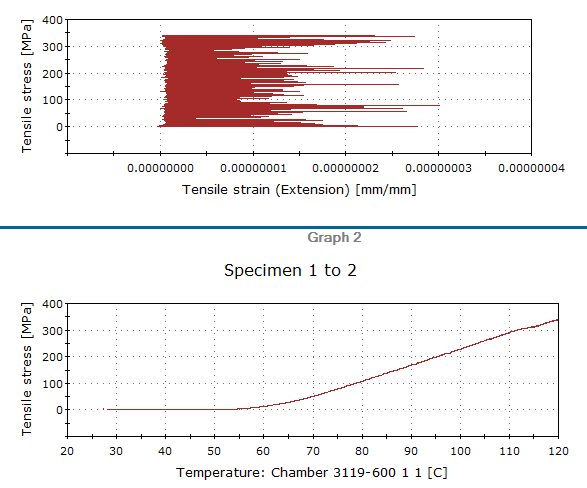
\includegraphics[width=\linewidth]{DYN1_single_temperature_0p.png}
\end{figure}

\textbf{Conclusion:} Since the stress increases when the wire is heated, there is contraction even in free-stress conditions.

\experiment{Instron: Shape memory effect}

\textbf{File:} dynalloy hybrid SME

\textbf{Objective:} Evaluate for 600MPa if the shape memory effect takes place

The wire was pre-heated to avoid any previous detwinning. From previous tensile tests, it seems that 600/700 MPa is the detwinning stress; hence the wire is loaded up to 600 MPa and unloaded. There will be residual strain. Afterwards the wire is heated above all transformation temperatures. When heating was necessary, the chamber door was closed and the SMA wire was heated. When closing the door, the tensile stress is slightly effected; hence, the experiment should start opened or only be closed when stress is equal to zero. Cooling is undertaken via free convection by opening the chamber door. However, such cooling is quite fast and the Instron stress controller has difficulty stabilizing it.

\begin{figure}[ht]
\centering
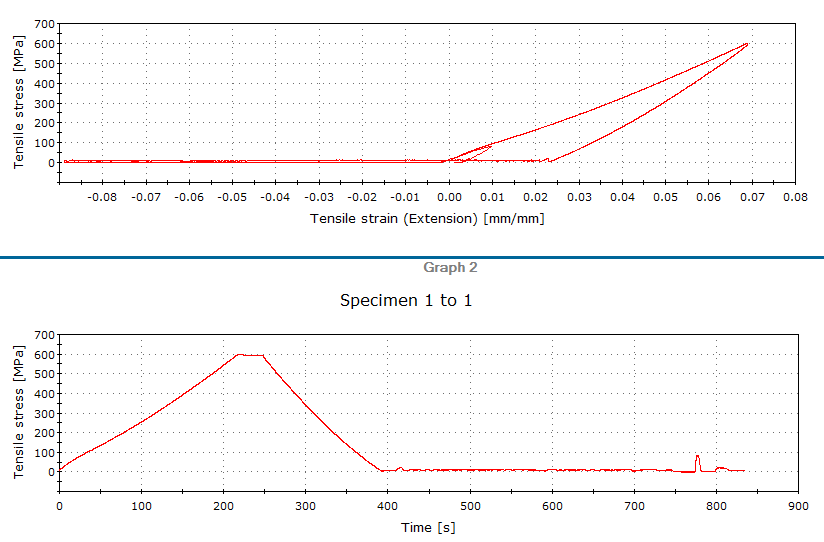
\includegraphics[width=\linewidth]{DYN1_hybrid_SME.png}
\end{figure}

\textbf{Conclusion:} There is a residual strain after loading up to 600 MPa. When heating the SMA shrinks to a length smaller than its original length. This indicates that the wire is \emph{two-way} material. (Lagoudas book, section 1.6 \cite{lagoudas_shape_2008})

%----------------------------------------------------------------------------------------
\labday{Thursday, 23 June 2016}

%-----------------------------------------
\experiment{Current Sensor: Calibration and first results of measurement.}

\textbf{File:} Current Sensor: Calibration. ???(IS THIS THE NAME OF THE FILE STORING THE DATA?!)

\textbf{Objective:} Are the sensor measurements reliable?

\textbf{Procedure for sensor calibration:}

\begin{itemize}
\item \textit{First Step}: Calibrate the output offset, with zero current on the sense lines(???), using the $V_{ref}$ trimpot. (WHAT IS A TRIMPOT?)

\item \textit{Second Step}: Using a known current, adjust the GAIN trimpot until the measured current showed in the monitor serial is similar to the current showed in the reference sensor.
\end{itemize}
\textbf{Conclusion:} 

\experiment{Instron: Cyclic loading (200MPa,400MPa, 600MPa, 400MPa) at room temperature.}

\textbf{Objective: } Verify influence of residual strain
\textbf{File:} DYN1 cyclic loading T0

\begin{figure}[ht]
\centering
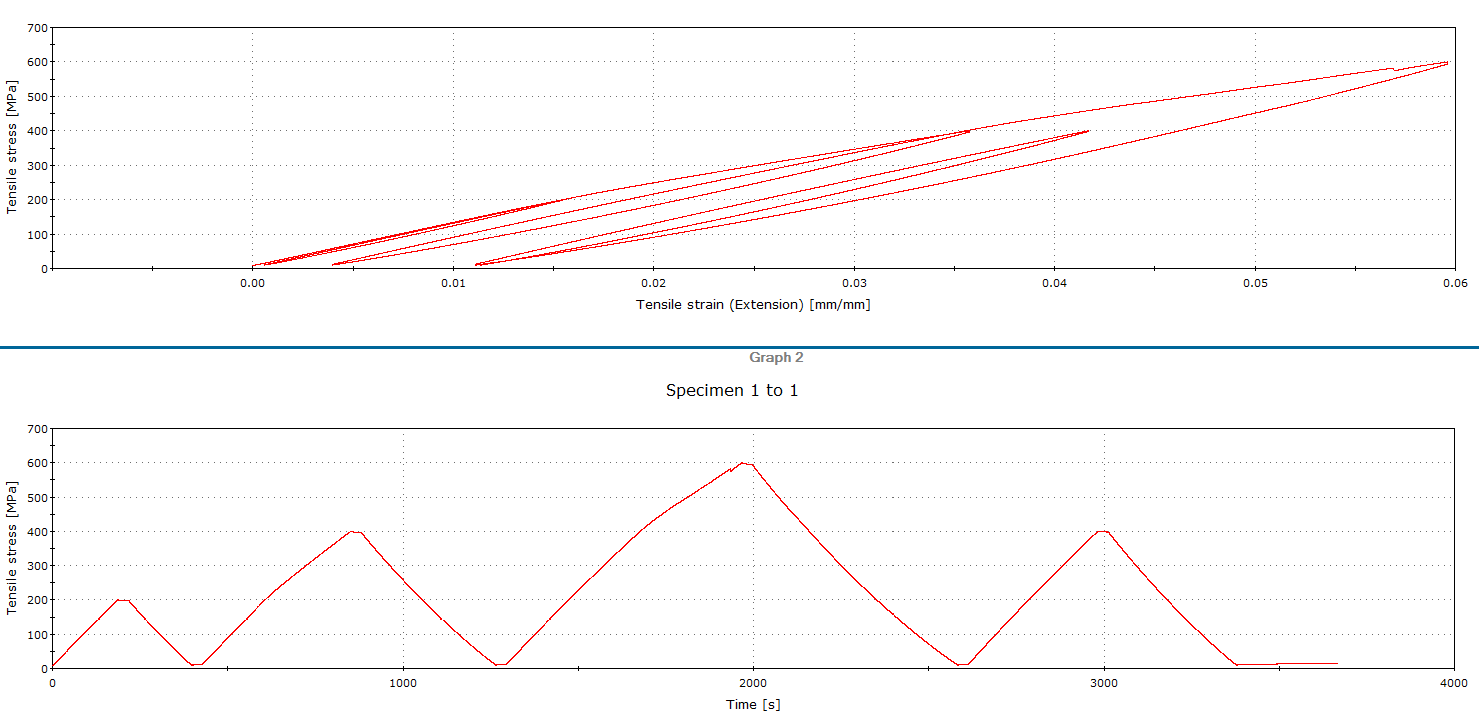
\includegraphics[width=\linewidth]{DYN1_cyclic_stress_T0.png}
\end{figure}

%------------------------------------------------------
\labday{Friday, 24 June 2016}

\experiment{Instron: Training - Cyclic heating at 200MPa.}

\textbf{File:} DYN1 cyclic temperature 200MPa

\textbf{Objective:} Train SMA wire

Previous training at 172 MPa did not stabilize SMA for other stresses. Thermal cycling at 600 MPa.
\begin{figure}[ht]
\centering
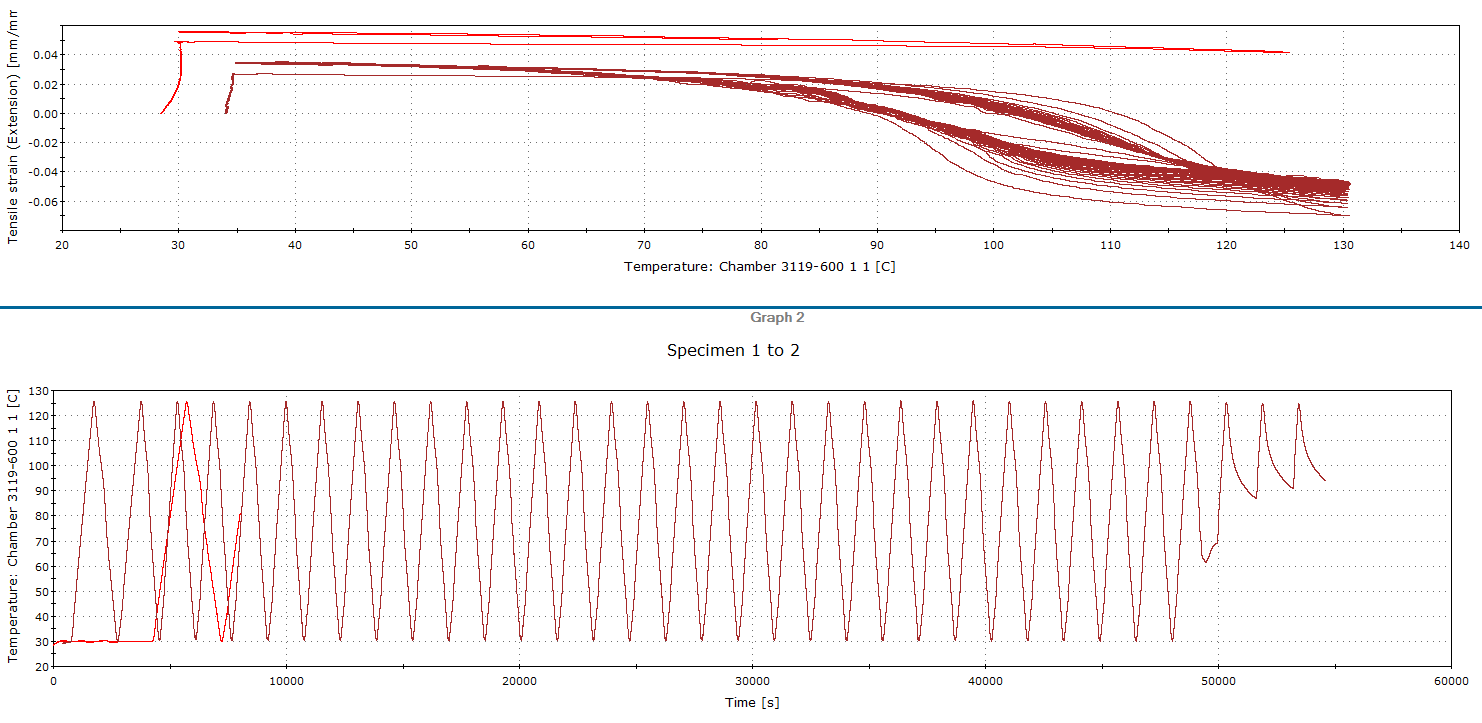
\includegraphics[width=\linewidth]{DYN1_cyclic_temperature_200MPa.png}
\end{figure}

\textbf{Conclusion:} With the current parameters, 30 cycles were successfully undertaken at 20MPa. The final cycles did not cool down because of lack of liquid nitrogen.

%------------------------------------------------------
\labday{Friday, 24 June 2016}

\experiment{Instron: Thermal cycling at constant stress (50MPa, 100MPa, 150MPa, 172MPa).}

A colocar imagens
%----------------------------------------------------------------------------------------
%	FORMULAE AND MEDIA RECIPES
%----------------------------------------------------------------------------------------

\labday{} % We don't want a date here so we make the labday blank

\begin{center}
\HRule \\[0.4cm]
{\huge \textbf{Formulae and Media Recipes}}\\[0.4cm] % Heading
\HRule \\[1.5cm]
\end{center}

%----------------------------------------------------------------------------------------
%	MEDIA RECIPES
%----------------------------------------------------------------------------------------

\newpage

\huge \textbf{Media} \\ \\

\normalsize \textbf{Media 1}\\
\begin{table}[H]
\begin{tabular}{l l l}
\toprule
\textbf{Compound} & \textbf{1L} & \textbf{0.5L}\\
\toprule
Compound 1 & 10g & 5g\\
Compound 2 & 20g & 10g\\
\bottomrule
\end{tabular}
\caption{Ingredients in Media 1.}
\label{tab:med1}
\end{table}

%-----------------------------------------

%\textbf{Media 2}\\ \\

%Description

%----------------------------------------------------------------------------------------
%	FORMULAE
%----------------------------------------------------------------------------------------

\newpage

\huge \textbf{Formulae} \\ \\

\normalsize \textbf{Formula 1 - Pythagorean theorem}\\ \\
$a^2 + b^2 = c^2$\\ \\

%-----------------------------------------

%\textbf{Formula X - Description}\\ \\

%Formula

%----------------------------------------------------------------------------------------

  \bibliographystyle{ieeetr}
  \bibliography{Master_thesis}
  
\end{document}